\section{Results}\label{sec:results}
The results presented in the following are based on simulations performed using the commercial simulator \questa\footnote{\texttt{QuestaSim-64, version 2020.4 linux\_x86\_64, Mentor Graphics Corporation}}. The printer and scoreboard logs were then post-processed with custom \emph{tcl} scripts, run within the simulator shell, and with \textsc{matlab} scripts.

\subsection{Intel's Pentium IV Adder}

\begin{figure}
    \centering
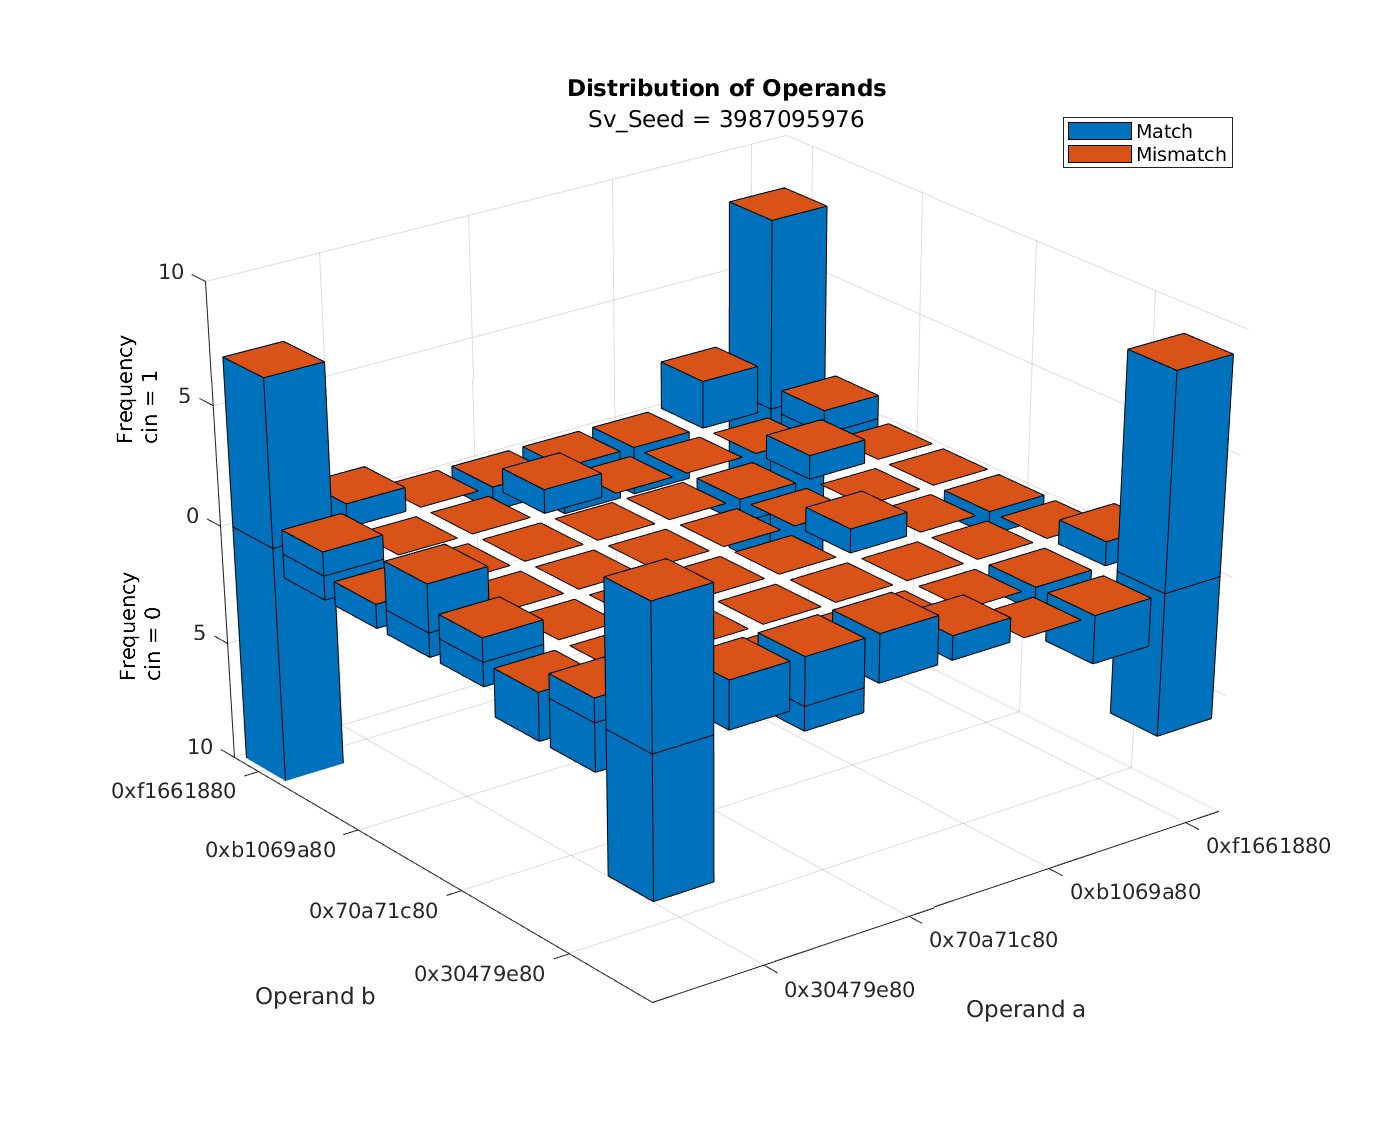
\includegraphics[width=.9\linewidth]{fig/p4_adder/p4_adder_nbit32_nbit_per_block4.eps}
    \caption{Visualization of the simulation logs for Intel's Pentium IV adder, parameterized with \textsc{nbit} $= 32$ and \textsc{nbit\_per\_block} $= 4$; 100 request transactions. The bar plots for the cases \svinline{cin} $= 0$ and \svinline{cin} $= 1$ are joined along the $\hat{z}$ direction to emphasize that the weighted distribution constraint was effective in skewing the stimulus towards the boundaries of the support set. No violations occurred.}
    \label{fig:p4-sim324}
\end{figure}

The verification of the Pentium IV adder was carried out across various parameterizations, as outlined below:
\begin{algorithmic}
\For{$i \in \{3, \dots, 7\}$}
    \For{$j \in \{2, \dots, i-1\}$}
        \State \textsc{nbit} $\gets 2^i$
            \State \textsc{nbit\_per\_block} $\gets 2^j$
    \EndFor
\EndFor
\end{algorithmic}
In each scenario, the test sequence was configured to generate 100 request transactions and the seed was randomly selected by the simulator. In all cases, the \ac{rtl} code coverage analysis reported full coverage and the \dut passed the test with the following scoreboard output:
\begin{minted}[bgcolor=backcolor, fontsize=\scriptsize]{text}
Scoreboard Summary:
  Transactions: 100 out of 100
  Errors      : 0
  Coverage    : 100.00%
\end{minted}

The post-processing of the logs, in the scenario where \textsc{nbit} is 32 and \textsc{nbit\_per\_block} is 4, is in~\cref{fig:p4-sim324}. This highlights how the weighted distribution constraint effectively skewed the stimulus towards the boundaries of the support set, a crucial aspect in covering the entire verification plan.

\subsection{Fixed-Size Windowed Register File}

\begin{figure}
\begin{adjustwidth}{-1cm}{-1cm}
    \centering
    \subfloat[][The pie chart illustrates that all operations were executed. Read and write operations were the most frequent, accounting for 2995 transactions. Surprisingly, \qty{14}{\percent} of the randomization attempts resulted in no operation being executed.\label{fig:wrf-sim_328884_ops}]
        {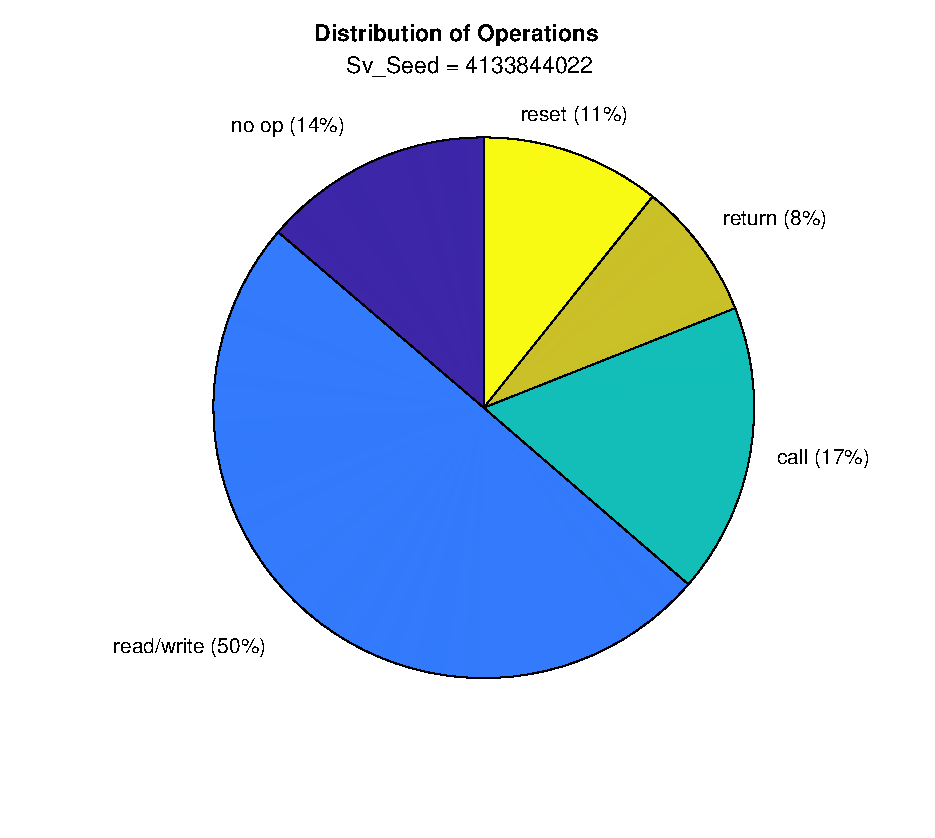
\includegraphics[width=.7\linewidth]{fig/windowed_rf/windowed_rf_nwindows4_ops.eps}}\vspace{.8cm}
    \subfloat[][Spill operations were triggered 196 times throughout the simulation.\label{fig:wrf-sim_328884_spill}]
        {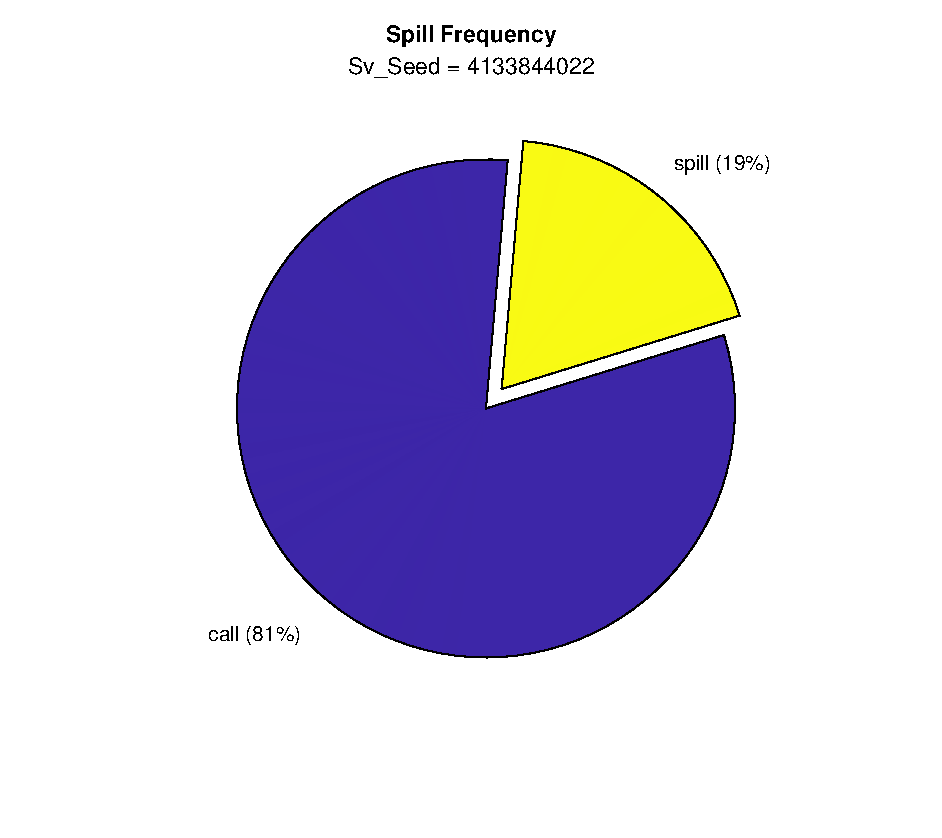
\includegraphics[width=.42\linewidth]{fig/windowed_rf/windowed_rf_nwindows4_spill.eps}}\quad
    \subfloat[][Fill operations were triggered 55 times throughout the simulation.\label{fig:wrf-sim_328884_fill}]
        {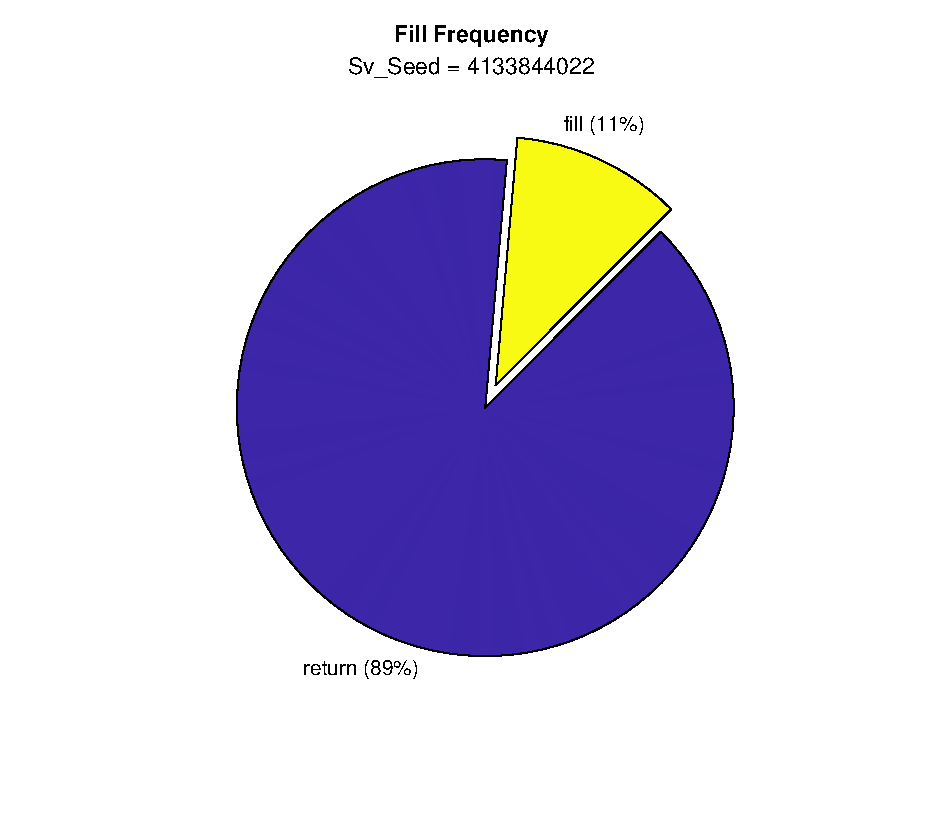
\includegraphics[width=.48\textwidth]{fig/windowed_rf/windowed_rf_nwindows4_fill.eps}}
\end{adjustwidth}
\caption{Visualization of the simulation logs for the fixed-size windowed register file, parameterized with \textsc{nbit} $= 32$, \textsc{nbit\_mem} $= 8$, \textsc{nglobals} $= 8$, \textsc{nlocals} $= 8$, and \textsc{nwindows} $= 4$; 2000 request transactions per test sequence, totaling 6000 transactions. No violations occurred.}
\label{fig:wrf-sim_328884}
\end{figure}

The verification of the fixed-size windowed register file was carried out across typical parameterization scenarios:
\begin{algorithmic}
\State \textsc{nbit} $\in \{8, 16, 32, 64\}$
\State \textsc{nbit\_mem} $\gets 8$ \Comment{memory management unit cycles depend on \textsc{nbit}}
\State \textsc{nglobals} $\in \{8, 10, 12\}$
\State \textsc{nlocals}  $\in \{8, 10, 12\}$
\State \textsc{nwindows} $\in \{4, 8, 16, 32\}$ \Comment{the smaller, the easier to trigger spill and fill}
\end{algorithmic}
In all scenarios, using 100 request transactions per test sequence, totaling 300 transactions, resulted in achieving a total function coverage ranging between \qty{74}{\percent} and \qty{95}{\percent}. Increasing the number of request transactions per test sequence to \num{2000} proved sufficient to achieve a coverage of \qty{100}{\percent} in most cases, while some scenarios required up to \num{5000} transactions per test sequence. To further stress both the testbench and the \dut, the number of request transactions was increased to \num{500000} per test sequence.

The \dut passed the test in all scenarios, but the \ac{rtl} code coverage analysis unearthed undesired redundancy in the \vhdlinline{transition_logic_p} of the \ac{fsm} that controls spill and fill operations. As shown in the following excerpt, the enumerated cases already cover all the enumeration constants, and the \vhdlinline{others} case prevents the correct interpretation of states and transitions during \questa compilation. 

\begin{minted}[bgcolor=backcolor, fontsize=\scriptsize]{vhdl}
  type state_t is (RUN, CWP_DOWN, SPILL_ONE, WAIT_SPILL, CWP_UP, WAIT_FILL, FILL_ONE);
  ...
  transition_logic_p : process (...) is
  begin

    case state is
      when RUN        => ...
      when CWP_DOWN   => ...
      when SPILL_ONE  => ...
      when WAIT_SPILL => ...
      when CWP_UP     => ...
      when WAIT_FILL  => ...
      when FILL_ONE   => ...
      
      when others     =>
        next_state <= RUN;

    end case;

  end process;
\end{minted}

The post-processing of the logs, in the scenario where \textsc{nbit} $= 32$, \textsc{nbit\_mem} $= 8$, \textsc{nglobals} $= 8$, \textsc{nlocals} $= 8$, and \textsc{nwindows} $= 4$, is in~\cref{fig:wrf-sim_328884}. This highlights the distribution of the executed operations, with an emphasis on call and return requests that triggered spill and fill operations.